% =====================================================================
% main.tex  -  Project report: Startup Incubation and Startup Management System
% Compile from the report/ folder:   pdflatex main.tex   (run it twice)
% =====================================================================
\documentclass[12pt,a4paper]{report}

% ---------- Page layout and fonts ----------
\usepackage[a4paper,margin=2.5cm]{geometry}   % margins
\usepackage[T1]{fontenc}                       % proper output of accented chars, underscores
\usepackage{lmodern}                           % clean, scalable font
\usepackage{microtype}                         % finer spacing -> fewer lines sticking into the margin
\setlength{\emergencystretch}{2em}             % allow a little extra word spacing when needed
\usepackage{setspace}                          % line spacing
\onehalfspacing

% ---------- Tables, figures, colours ----------
\usepackage{graphicx}                          % \includegraphics for screenshots
\usepackage{booktabs}                          % professional table rules
\usepackage{tabularx}                          % tables that fill the text width
\usepackage{longtable}                         % tables that can break across pages
\usepackage{array}
\usepackage{float}                             % [H] placement option
\usepackage[font=small,labelfont=bf]{caption}  % caption style
\usepackage[table]{xcolor}                     % colours (also for table rows)
\usepackage{enumitem}                          % compact lists
\setlist{itemsep=2pt,topsep=4pt}

% ---------- Diagrams ----------
\usepackage{tikz}
\usetikzlibrary{positioning,arrows.meta,shapes.geometric,fit,calc}

% ---------- Code listings (SQL and Python) ----------
\usepackage{listings}
\definecolor{codebg}{RGB}{247,247,247}
\definecolor{codekw}{RGB}{0,70,160}
\definecolor{codecomment}{RGB}{0,120,60}
\definecolor{codestring}{RGB}{160,40,40}
\lstdefinestyle{base}{
  basicstyle=\ttfamily\footnotesize,
  backgroundcolor=\color{codebg},
  keywordstyle=\color{codekw}\bfseries,
  commentstyle=\color{codecomment}\itshape,
  stringstyle=\color{codestring},
  frame=single, rulecolor=\color{gray!50},
  breaklines=true, columns=fullflexible, keepspaces=true,
  showstringspaces=false, tabsize=4,
  numbers=left, numberstyle=\tiny\color{gray}, numbersep=6pt,
  xleftmargin=1.5em, framexleftmargin=1.5em,
  captionpos=b, aboveskip=8pt, belowskip=8pt
}
\lstdefinestyle{sql}{style=base, language=SQL, morekeywords={REFERENCES,RETURNING,ILIKE,
  CASCADE,RESTRICT,GENERATED,ALWAYS,IDENTITY,VIEW,REPLACE,EXISTS,NULLIF,COALESCE,
  STRING_AGG,TRUNCATE,BEGIN,COMMIT,ROLLBACK,ANY,FILTER,INDEX,CONSTRAINT,CHECK,UNIQUE,
  BETWEEN,FOR,LEFT,INNER,JOIN,HAVING,CASE,WHEN,THEN,ELSE,END}}
\lstdefinestyle{py}{style=base, language=Python}
\renewcommand{\lstlistingname}{Listing}

% ---------- Header and footer ----------
\usepackage{fancyhdr}
\pagestyle{fancy}
\fancyhf{}
\fancyhead[L]{\small\nouppercase{\leftmark}}
\fancyfoot[C]{\thepage}
\renewcommand{\headrulewidth}{0.4pt}
\setlength{\headheight}{15pt}
\fancypagestyle{plain}{\fancyhf{}\fancyfoot[C]{\thepage}\renewcommand{\headrulewidth}{0pt}}

% ---------- Short commands used in the text ----------
\newcommand{\code}[1]{\texttt{#1}}             % inline code / table names

% ---------- Hyperlinks (load last) ----------
\usepackage[hidelinks]{hyperref}

% =====================================================================
% FILL IN YOUR DETAILS HERE
% =====================================================================
% Separate several names with \\ .  Do NOT start a name with "[" right after \\ ,
% because LaTeX reads \\[...] as "line break + extra space" and stops with an error.
\newcommand{\studentnames}{Student Name 1 \\ Student Name 2}
\newcommand{\rollnumbers}{Roll No. 1 \\ Roll No. 2}
\newcommand{\coursename}{Database Systems (DBS)}
\newcommand{\instructor}{[Name of Course Instructor]}
\newcommand{\department}{[Department Name]}
\newcommand{\institution}{[Institution Name]}
\newcommand{\submissiondate}{[Month Year]}

\begin{document}

% =====================================================================
% Title page
% =====================================================================
\begin{titlepage}
  \centering
  \vspace*{1cm}
  {\large \institution \par}
  {\large \department \par}
  \vspace{1.5cm}
  {\large Course Project Report \par}
  {\large \coursename \par}
  \vspace{1.5cm}
  \rule{\textwidth}{1pt}\par\vspace{0.4cm}
  {\LARGE\bfseries Startup Incubation and\\[4pt] Startup Management System \par}
  \vspace{0.3cm}
  {\large A database-driven application using Python, PostgreSQL and Streamlit \par}
  \vspace{0.4cm}\rule{\textwidth}{1pt}
  \vfill
  \begin{tabular}{ll}
    \textbf{Submitted by:} & \begin{tabular}[t]{@{}l@{}}\studentnames\end{tabular} \\[1.2em]
    \textbf{Roll number:}  & \begin{tabular}[t]{@{}l@{}}\rollnumbers\end{tabular} \\[1.2em]
    \textbf{Submitted to:} & \instructor \\[1.2em]
  \end{tabular}
  \vfill
  {\large \submissiondate \par}
\end{titlepage}

% =====================================================================
% Front matter: abstract and tables of contents (roman page numbers)
% =====================================================================
\pagenumbering{roman}

\chapter*{Abstract}
\addcontentsline{toc}{chapter}{Abstract}
Startup incubation centres admit early-stage startups into a support programme, evaluate
their applications, assign mentors and track their progress. When this work is done with
spreadsheets and e-mail, the same data is stored in many places, rules such as ``only admitted
startups receive mentors'' are not enforced, and simple management questions require manual
counting.

This project designs and implements a database-driven application that solves these problems.
The database, implemented in PostgreSQL, consists of nine relations---\code{startup},
\code{founder}, \code{application}, \code{evaluator}, \code{evaluation}, \code{incubation},
\code{mentor}, \code{mentorship} and \code{milestone}---derived from an ER model and shown to be
in Boyce--Codd Normal Form (and therefore in 3NF). Integrity is enforced inside the database by
primary keys, foreign keys with deliberate \code{ON DELETE} rules, \code{NOT NULL},
\code{UNIQUE} and \code{CHECK} constraints, and a partial unique index. Multi-step operations,
such as admitting a startup into incubation, are executed as transactions.

The application, written in Python with Streamlit and psycopg, provides five functional
modules---Startup, Application, Evaluation, Mentor and Progress Management---and separate views
for four user roles: Administrator, Startup/Founder, Evaluator and Mentor. It uses 21 SQL queries
and two views covering joins, aggregates, \code{GROUP BY}/\code{HAVING}, subqueries, correlated
subqueries and \code{EXISTS}. An automated test suite of 56 test cases and a database constraint
test script were executed, and all tests passed.

\tableofcontents
\listoffigures
\listoftables
\lstlistoflistings

% =====================================================================
% Main chapters (arabic page numbers)
% =====================================================================
\clearpage
\pagenumbering{arabic}

% =====================================================================
% Chapter 1: Introduction
% =====================================================================
\chapter{Introduction}
\label{ch:introduction}

\section{Background}
A startup incubation centre supports early-stage companies for a fixed period. A typical
centre carries out the following activities:
\begin{enumerate}
  \item keeping records of registered startups and their founders;
  \item receiving applications for its incubation programme;
  \item having expert evaluators score each application;
  \item admitting the best applicants into incubation;
  \item assigning mentors to admitted startups; and
  \item tracking each admitted startup's progress through milestones.
\end{enumerate}
Each activity produces data that depends on the data of earlier activities: an evaluation
belongs to an application, an incubation is created from an accepted application, and
mentors and milestones belong to an incubation. This chain of dependent data makes the domain
a good fit for a relational database.

\section{Problem Statement}
\label{sec:problem}
Small incubation centres frequently manage this process with spreadsheets, e-mail threads and
paper forms. This causes four concrete problems:
\begin{itemize}
  \item \textbf{Redundancy and update anomalies.} A startup's details are re-typed in several
        sheets (applications, evaluations, mentoring). When one copy is changed, the others
        become inconsistent.
  \item \textbf{No enforcement of business rules.} Nothing prevents a mentor from being
        ``assigned'' to a startup that was never admitted, or a score of 150 out of 100 being
        recorded.
  \item \textbf{Broken references.} An evaluation can refer to an application that has been
        deleted or never existed.
  \item \textbf{Slow reporting.} Questions such as ``What is the average score of each
        applicant?'' or ``Which mentor guides the most startups?'' must be answered by manual
        counting.
\end{itemize}

\section{Need for the System}
A relational database with an application on top of it addresses each of these problems:
\begin{itemize}
  \item \textbf{Single source of truth:} each fact is stored once, in a normalized schema.
  \item \textbf{Integrity enforced by the database itself:} primary keys, foreign keys,
        \code{NOT NULL}, \code{UNIQUE} and \code{CHECK} constraints reject invalid data even if
        the user interface has a defect.
  \item \textbf{Consistent multi-step operations:} transactions guarantee that, for example,
        accepting an application and creating its incubation record either both happen or
        neither happens.
  \item \textbf{Instant reports:} joins, aggregate functions and subqueries answer management
        questions directly from the stored data.
\end{itemize}

\section{Objectives}
\label{sec:objectives}
The objectives of the project are:
\begin{enumerate}
  \item To design a normalized relational database (at least 3NF) for the incubation process.
  \item To enforce data integrity using appropriate database constraints.
  \item To provide a working user interface through which users perform \code{INSERT},
        \code{UPDATE}, \code{DELETE} and \code{SELECT} operations in every module.
  \item To implement the application life cycle: submission $\rightarrow$ evaluation
        $\rightarrow$ decision $\rightarrow$ incubation.
  \item To support mentor assignment and milestone-based progress tracking for incubated
        startups.
  \item To generate meaningful reports using joins, aggregates, \code{GROUP BY}/\code{HAVING},
        subqueries and views.
  \item To demonstrate transactions for multi-step operations.
\end{enumerate}

\section{Scope of the Project}
\label{sec:scope}
\textbf{In scope.} Five functional modules (Startup, Application, Evaluation, Mentor and
Progress Management), the reports listed in Section~\ref{sec:reports}, the constraints implied
by the business rules, a role-based user interface, a locally hosted PostgreSQL database and
realistic sample data (10 startups, 18 founders, 10 applications, 20 evaluations, 5 evaluators,
6 mentors, 5 incubations and 15 milestones).

\textbf{Out of scope.} The following were deliberately excluded to keep the project focused on
database design and implementation: user login and authentication; payments, funding rounds
and investor portals; notifications, e-mail and chat; AI-based recommendations; multiple
incubation centres; resource or office-space allocation; file uploads; and cloud deployment.

\section{Users of the System}
\label{sec:users}
The application offers a separate set of screens (tabs) for each of four roles,
summarised in Table~\ref{tab:users}.

\begin{table}[H]
  \centering
  \caption{Users of the system and what each role can do}
  \label{tab:users}
  \begin{tabularx}{\textwidth}{@{}lX@{}}
    \toprule
    \textbf{Role} & \textbf{Capabilities} \\
    \midrule
    Administrator      & Register and maintain startups and founders; maintain evaluators and
                         mentors; change application status; admit startups to incubation;
                         assign mentors; create milestones; view all reports. \\
    Startup / Founder  & View and update its own startup; submit applications; track
                         application status and read evaluator feedback; view its milestones
                         and progress. \\
    Evaluator          & See the applications under review that he or she has not yet
                         evaluated; record a score and feedback; view past evaluations. \\
    Mentor             & See the startups he or she mentors; add mentorship remarks; update
                         the milestone status of those startups only. \\
    \bottomrule
  \end{tabularx}
\end{table}

The role is chosen from a ``View as'' selector in the sidebar, after which the user selects
which startup, evaluator or mentor he or she is. Every query on those screens is then filtered
by the selected identifier (for example \code{WHERE evaluator\_id = \%s}). This is a user
interface feature that shows different users different parts of the same database; it is
\emph{not} an authentication mechanism, which is outside the scope of the project.

% =====================================================================
% Chapter 2: Requirements, Technology and Architecture
% =====================================================================
\chapter{Requirements and System Architecture}
\label{ch:requirements}

\section{Functional Modules}
\label{sec:modules}
The application is divided into five functional modules. A module represents a piece of
functionality, not a single table; most modules use several tables
(Table~\ref{tab:modules}).

\begin{table}[H]
  \centering
  \caption{Functional modules and the tables each one uses}
  \label{tab:modules}
  \begin{tabularx}{\textwidth}{@{}lXl@{}}
    \toprule
    \textbf{Module} & \textbf{Purpose} & \textbf{Tables used} \\
    \midrule
    1. Startup Management     & Register, view, search, update and delete startups and their founders
                              & \code{startup}, \code{founder} \\
    2. Application Management & Submit applications, track and change their status, admit
                                accepted startups into incubation
                              & \code{application}, \code{evaluation}, \code{incubation} \\
    3. Evaluation Management  & Maintain evaluators, record scores and feedback, view results
                              & \code{evaluator}, \code{evaluation}, \code{application} \\
    4. Mentor Management      & Maintain mentors, assign them to incubated startups, maintain
                                mentorship records
                              & \code{mentor}, \code{mentorship}, \code{incubation} \\
    5. Progress Management    & Create milestones, update their status, track progress
                              & \code{milestone}, \code{incubation}, \code{mentorship} \\
    \bottomrule
  \end{tabularx}
\end{table}

\section{Functional Requirements}
\label{sec:fr}
Each requirement has an identifier (FR-$x.y$) so that it can be traced to tables, queries and
test cases in later chapters.

\begin{longtable}{@{}lp{0.80\textwidth}@{}}
  \caption{Functional requirements}\label{tab:fr}\\
  \toprule
  \textbf{ID} & \textbf{Requirement} \\
  \midrule
  \endfirsthead
  \toprule
  \textbf{ID} & \textbf{Requirement} \\
  \midrule
  \endhead
  \multicolumn{2}{@{}l}{\textit{Module 1 --- Startup Management}} \\
  FR-1.1 & Register a new startup. \\
  FR-1.2 & Add one or more founders to a startup. \\
  FR-1.3 & View the list of startups, with search by name or city and filter by sector. \\
  FR-1.4 & View the full details of one startup, including its founders. \\
  FR-1.5 & Update startup and founder information. \\
  FR-1.6 & Delete a startup only where appropriate (see BR-9). \\
  \midrule
  \multicolumn{2}{@{}l}{\textit{Module 2 --- Application Management}} \\
  FR-2.1 & Submit an incubation application for a registered startup. \\
  FR-2.2 & View all applications, with filter by status. \\
  FR-2.3 & Track the status of a given application. \\
  FR-2.4 & Update application status (Submitted $\rightarrow$ Under Review $\rightarrow$ Accepted / Rejected). \\
  FR-2.5 & On acceptance, admit the startup into incubation as a single transaction. \\
  \midrule
  \multicolumn{2}{@{}l}{\textit{Module 3 --- Evaluation Management}} \\
  FR-3.1 & Add, view, update and delete evaluators. \\
  FR-3.2 & Record an evaluation score for an application by an evaluator. \\
  FR-3.3 & Store written feedback with each evaluation. \\
  FR-3.4 & View evaluation results per application (each score, average, highest, lowest). \\
  \midrule
  \multicolumn{2}{@{}l}{\textit{Module 4 --- Mentor Management}} \\
  FR-4.1 & Add, view, update and delete mentors. \\
  FR-4.2 & Assign a mentor to an admitted (incubated) startup. \\
  FR-4.3 & View mentor assignments by mentor and by startup. \\
  FR-4.4 & Maintain mentorship records (assignment date, end date, status, remarks). \\
  \midrule
  \multicolumn{2}{@{}l}{\textit{Module 5 --- Progress Management}} \\
  FR-5.1 & Create milestones for an incubated startup. \\
  FR-5.2 & Update milestone status (Pending $\rightarrow$ In Progress $\rightarrow$ Completed). \\
  FR-5.3 & Record the completion date when a milestone is completed. \\
  FR-5.4 & View the progress of a startup (completed versus total milestones, percentage). \\
  FR-5.5 & Identify overdue milestones. \\
  \bottomrule
\end{longtable}

\section{Business Rules}
\label{sec:br}
Business rules are the real-world rules that the stored data must obey. During design, each
rule becomes a constraint, a relationship cardinality or a transaction
(Table~\ref{tab:br}). How each rule is enforced is explained in Chapter~3.

\begin{table}[H]
  \centering
  \caption{Business rules}
  \label{tab:br}
  \begin{tabularx}{\textwidth}{@{}lX@{}}
    \toprule
    \textbf{ID} & \textbf{Rule} \\
    \midrule
    BR-1  & A startup has one or more founders; a founder belongs to exactly one startup. \\
    BR-2  & Startup names and e-mail addresses are unique. \\
    BR-3  & A startup may apply several times (e.g.\ after a rejection) but may have only one
            open (Submitted or Under Review) application at a time. \\
    BR-4  & Application status is one of Submitted, Under Review, Accepted or Rejected. \\
    BR-5  & An application may be evaluated by many evaluators, but each evaluator evaluates a
            given application at most once. \\
    BR-6  & An evaluation score is a whole number from 0 to 100. \\
    BR-7  & An application can be accepted only if it has at least one evaluation; accepting it
            creates an incubation record, and both changes succeed or fail together. \\
    BR-8  & Mentors can be assigned only to incubated startups; a mentor can guide many startups
            and a startup can have many mentors. \\
    BR-9  & A startup with application history cannot be deleted; a startup without applications
            can be deleted together with its founders. \\
    BR-10 & A milestone is Pending, In Progress or Completed; a completion date exists if and only
            if the status is Completed. \\
    BR-11 & Dates must be logical (for example, the expected end date is after the start date). \\
    \bottomrule
  \end{tabularx}
\end{table}

\section{Reports and Outputs}
\label{sec:reports}
The application produces the reports in Table~\ref{tab:reports}. Each report also exercises a
particular SQL concept from the course.

\begin{table}[H]
  \centering
  \caption{Reports produced by the application}
  \label{tab:reports}
  \begin{tabularx}{\textwidth}{@{}lXl@{}}
    \toprule
    \textbf{ID} & \textbf{Report} & \textbf{Main SQL concept} \\
    \midrule
    R1  & Startups per sector                                  & \code{COUNT}, \code{GROUP BY} \\
    R2  & Applications and funding requested by status         & \code{COUNT}, \code{SUM}, \code{AVG} \\
    R3  & Evaluation summary per application                   & \code{AVG}, \code{MIN}, \code{MAX}, joins \\
    R4  & Applications scoring above the overall average       & subquery in \code{HAVING} \\
    R5  & Applications not yet evaluated                       & \code{LEFT JOIN \ldots\ IS NULL} \\
    R6  & Mentor workload (active startups per mentor)         & \code{LEFT JOIN}, \code{COUNT} \\
    R7  & Incubated startups without an active mentor          & \code{LEFT JOIN} \\
    R8  & Progress per startup (\% milestones completed)       & \code{CASE} inside \code{SUM} \\
    R9  & Overdue milestones                                   & date arithmetic \\
    R10 & Highest-scoring evaluation of each application       & correlated subquery \\
    R11 & Incubation dashboard                                 & view \\
    \bottomrule
  \end{tabularx}
\end{table}

\section{Non-Functional Requirements}
\begin{itemize}
  \item The application runs locally on a single Windows computer.
  \item Data integrity is enforced in the database, not only in the user interface.
  \item All SQL is written by hand (no ORM) and every user-supplied value is passed as a query
        parameter, which prevents SQL injection.
  \item The code is kept simple and readable, with one file per functional module.
\end{itemize}

\section{Technology Stack}
\label{sec:tech}
\begin{table}[H]
  \centering
  \caption{Technology stack}
  \label{tab:tech}
  \begin{tabularx}{\textwidth}{@{}llX@{}}
    \toprule
    \textbf{Component} & \textbf{Version} & \textbf{Role in the project} \\
    \midrule
    PostgreSQL   & 18.6   & Relational database server: tables, constraints, views, transactions \\
    Python       & 3.14   & Application logic \\
    psycopg      & 3.3.8  & Database driver: sends SQL and parameters to PostgreSQL and returns rows \\
    Streamlit    & 1.67.0 & Web user interface: forms, tables, charts and tabs in the browser \\
    psql, pgAdmin 4 & ---  & Running SQL scripts and inspecting the database \\
    \bottomrule
  \end{tabularx}
\end{table}

\section{System Architecture}
\label{sec:architecture}
The application follows a simple layered architecture (Figure~\ref{fig:architecture}). The
user works in a web browser. Every interaction re-runs the Streamlit script \code{app.py},
which shows the tabs for the selected role and calls a function in the corresponding module
file. The module function builds an SQL statement with \code{\%s} placeholders and calls
\code{db.py}, the only file that communicates with PostgreSQL. \code{db.py} uses psycopg to send
the SQL and its parameters to the database server, which checks all constraints, executes the
statement and returns rows or an error. The result travels back up the same path and is
displayed on the screen.

\begin{figure}[H]
  \centering
  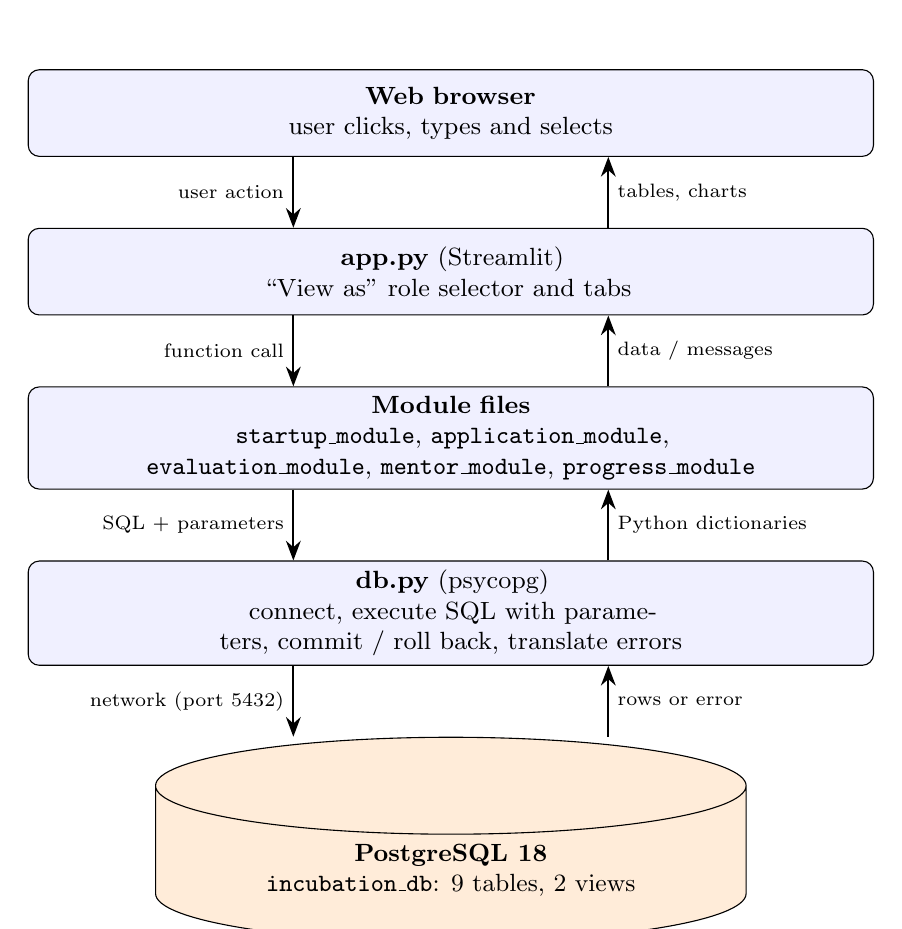
\begin{tikzpicture}[
      layer/.style={draw, rounded corners, fill=blue!6, text width=10.5cm,
                    minimum height=1.1cm, align=center, font=\small},
      db/.style={draw, cylinder, shape border rotate=90, aspect=0.25, fill=orange!15,
                 minimum width=7.5cm, minimum height=1.6cm, align=center, font=\small},
      arr/.style={-{Stealth[length=2.5mm]}, thick},
      lbl/.style={font=\scriptsize, fill=white, inner sep=1pt}]
    \node[layer] (browser) {\textbf{Web browser}\\ user clicks, types and selects};
    \node[layer, below=0.9cm of browser] (app)
      {\textbf{app.py} (Streamlit)\\ ``View as'' role selector and tabs};
    \node[layer, below=0.9cm of app] (modules)
      {\textbf{Module files}\\ \code{startup\_module}, \code{application\_module},
       \code{evaluation\_module}, \code{mentor\_module}, \code{progress\_module}};
    \node[layer, below=0.9cm of modules] (dbpy)
      {\textbf{db.py} (psycopg)\\ connect, execute SQL with parameters, commit / roll back,
       translate errors};
    \node[db, below=0.9cm of dbpy] (pg)
      {\textbf{PostgreSQL 18}\\ \code{incubation\_db}: 9 tables, 2 views};

    \draw[arr] ([xshift=-2cm]browser.south) -- node[lbl,left=2pt]{user action} ([xshift=-2cm]app.north);
    \draw[arr] ([xshift=-2cm]app.south) -- node[lbl,left=2pt]{function call} ([xshift=-2cm]modules.north);
    \draw[arr] ([xshift=-2cm]modules.south) -- node[lbl,left=2pt]{SQL + parameters} ([xshift=-2cm]dbpy.north);
    \draw[arr] ([xshift=-2cm]dbpy.south) -- node[lbl,left=2pt]{network (port 5432)} ([xshift=-2cm]pg.north);

    \draw[arr] ([xshift=2cm]pg.north) -- node[lbl,right=2pt]{rows or error} ([xshift=2cm]dbpy.south);
    \draw[arr] ([xshift=2cm]dbpy.north) -- node[lbl,right=2pt]{Python dictionaries} ([xshift=2cm]modules.south);
    \draw[arr] ([xshift=2cm]modules.north) -- node[lbl,right=2pt]{data / messages} ([xshift=2cm]app.south);
    \draw[arr] ([xshift=2cm]app.north) -- node[lbl,right=2pt]{tables, charts} ([xshift=2cm]browser.south);
  \end{tikzpicture}
  \caption{Layered architecture of the application}
  \label{fig:architecture}
\end{figure}

\section{Project Structure}
\label{sec:structure}
Each file has a single responsibility (Table~\ref{tab:structure}).

\begin{table}[H]
  \centering
  \caption{Project files and their responsibilities}
  \label{tab:structure}
  \begin{tabularx}{\textwidth}{@{}lX@{}}
    \toprule
    \textbf{File} & \textbf{Responsibility} \\
    \midrule
    \code{sql/01\_schema.sql}          & Creates the 9 tables, their constraints and the partial unique index \\
    \code{sql/02\_sample\_data.sql}    & Inserts the sample data in a single transaction \\
    \code{sql/03\_constraint\_tests.sql} & Deliberately violates each constraint and demonstrates \code{INSERT}, \code{UPDATE} and \code{DELETE} (rolled back at the end) \\
    \code{sql/04\_queries.sql}         & The report queries Q1--Q19 \\
    \code{sql/05\_views.sql}           & The two views and queries Q20--Q21 that use them \\
    \code{app/db.py}                   & The only file that talks to PostgreSQL \\
    \code{app/app.py}                  & Entry point: role selector and tab layout \\
    \code{app/startup\_module.py}      & Module 1: database functions and screens \\
    \code{app/application\_module.py}  & Module 2, including the admission transaction \\
    \code{app/evaluation\_module.py}   & Module 3 \\
    \code{app/mentor\_module.py}       & Module 4 \\
    \code{app/progress\_module.py}     & Module 5 \\
    \code{tests/test\_app.py}          & Automated test suite (56 test cases) \\
    \bottomrule
  \end{tabularx}
\end{table}

% Added in the next steps:
% \input{chapters/03_database_design}
% \input{chapters/04_normalization}
% \input{chapters/05_implementation}
% \input{chapters/06_testing}
% \input{chapters/07_conclusion}

\end{document}
